% !TeX program = pdfLaTeX
\documentclass[12pt]{article}
\usepackage{amsmath}
\usepackage{amsthm}
\usepackage{graphicx,psfrag,epsf}
\usepackage{enumerate}
\usepackage{natbib}
\usepackage{booktabs}
\usepackage{longtable}
\usepackage{array}
\usepackage{multirow}
\usepackage[table]{xcolor}
\usepackage{wrapfig}
\usepackage{float}
\usepackage{colortbl}
\usepackage{hyperref}
\usepackage{pdflscape}
\usepackage{tabu}
\usepackage{threeparttable}

\usepackage{url} % not crucial - just used below for the URL

%\pdfminorversion=4
% NOTE: To produce blinded version, replace "0" with "1" below.
\newcommand{\blind}{0}

% DON'T change margins - should be 1 inch all around.
\addtolength{\oddsidemargin}{-.5in}%
\addtolength{\evensidemargin}{-.5in}%
\addtolength{\textwidth}{1in}%
\addtolength{\textheight}{1.3in}%
\addtolength{\topmargin}{-.8in}%

\newenvironment{definition}[1]% environment name 
{% begin code 
  \par\vspace{.75\baselineskip}\noindent 
  \textbf{Definition (#1)}\begin{itshape}% 
  \par\vspace{.5\baselineskip}\noindent\ignorespaces 
}% 
{% end code 
  \end{itshape}\ignorespacesafterend 
}

\providecommand{\tightlist}{%
  \setlength{\itemsep}{0pt}\setlength{\parskip}{0pt}}

\begin{document}

\def\spacingset#1{\renewcommand{\baselinestretch}%
{#1}\small\normalsize} \spacingset{1}


%%%%%%%%%%%%%%%%%%%%%%%%%%%%%%%%%%%%%%%%%%%%%%%%%%%%%%%%%%%%%%%%%%%%%%%%%%%%%%

\if0\blind
{
  \title{\bf Adaption of the Chumbley Score to matching of bullet striation marks}

  \author{
        Ganesh Krishnan \thanks{The authors gratefully acknowledge \ldots{}} \\
    Department of Statistics, Iowa State University\\
     and \\     Heike Hofmann \\
    Department of Statistics and CSAFE, Iowa State University\\
      }
  \maketitle
} \fi

\if1\blind
{
  \bigskip
  \bigskip
  \bigskip
  \begin{center}
    {\LARGE\bf Adaption of the Chumbley Score to matching of bullet striation marks}
  \end{center}
  \medskip
} \fi

\bigskip
\begin{abstract}

\end{abstract}

\noindent%
{\it Keywords:} 3 to 6 keywords, that do not appear in the title
\vfill

\newpage
\spacingset{1.45} % DON'T change the spacing!

\newcommand{\hh}[1]{{\textcolor{orange}{#1}}}
\newcommand{\gk}[1]{{\textcolor{green}{#1}}}
\newcommand{\cited}[1]{{\textcolor{red}{#1}}}

\tableofcontents
\newpage

\section{Introduction and Background}\label{introduction-and-background}

\subsection{Motivation}\label{motivation}

Same source analyses are a major part of an Forensic Toolmark Examiner's
job. In current practice examiners make these comparisons by visual
inspection under a comparison microscope and come to one of the
following four conclusions: identification, inconclusive, elimination or
unsuitable for examination\textasciitilde{}\citep{afte-toolmarks1998}.
These conclusions are made on the basis of ``unique surface contours''
of the two toolmarks being in ``sufficient agreement''
\citep{afte-toolmarks1998}. AFTE describes the term ``sufficient
agreement'' as the possibility of another tool producing the markings
under comparison, as practically impossible \citep{afte-toolmarks1998}.
This subjectivity in the assessment as well as the lack of error rates
are the main points of criticisms first raised by the National Research
Council in 2009 \citep{NAS:2009} and later emphasized further by the
President's Council of Advisors on Science and Technology
\citep{pcast2016}.

Technological advances, such as profilometers and confocal microscopy
allow to measure 3D surfaces in a high-resolution digitized form. This
technology has become more accessible over the last decade, and has made
its way into topological images of ballistics evidence, such as bullet
lands and breech faces
\citep{DeKinder1, DeKinder2, Bachrach1, vorburger2016}. Digitized images
of 3D surfaces of form the data basis of statistical analysis of
toolmarks. A statistical approach based on data removes both
subjectivity from the assessment and allows a quantification of error
rates for both false positive and false negative identifications.

\hh{In the next page and a half it is easy to lose the red line. It might help to include a table with an overview.
The table should include the reference to the paper, the data used, the statistical method and the associated error rates.}
Various toolmarks have been studied in the literature:
\citet{manytoolmarks1} and \citet{chumbley} have been analyzing
screwdriver marks digitized using a profilometer; \citet{manytoolmarks2}
have investigated 3D marks from screwdriver, tongue and groove pliers
captured using a confocal microscope; \citet{afte-chumbley} have been
investigated digitized marks from slip-joint pliers generated by a
surface profilometer.

\hh{We need an additional sentence here to get from the data to the statistical methods ... }
\citet{manytoolmarks2} define a relative distance metric and use it as
similarity measure between two toolmarks. \citet{manytoolmarks1} extract
many small segments in the markings of two toolmarks and compare
similiarity using a maximum pearson correlation coefficient. The
Chumbley scoring method, first introduced by \citet{chumbley}, uses a
similar but more extensive framework based on a Mann-Whitney U test of
the resulting correlation coefficients. This approach is
non-deterministic, because segments are chosen randomly. \citep{hadler}
make the score deterministic for each pair of toolmarks by choosing
segments for comparison systematically. This approach also ensures
independence between segements of striae. In this paper, we are
investigating the applicability of the Chumbley scoring method by
\citet{hadler} to assess striation marks on bullet lands for same-source
identification.

Striation marks on bullets are made by impurities in the barrel. As the
bullet travels through the barrel, these imperfections leave
``scratches'' on the bullet surface. Typically, only striation marks in
the land engraved areas (LEAs) are considered \citet{afte-article1992}.
Bullet lands are depressed areas between the grooves made by the rifling
action of the barrel. Compared to toolmarks made by screwdrivers
striation marks on bullets are typically much smaller, both in length
and in width. Bullets also have a curved cross-sectional topography.
Figure \ref{fig:rgl} shows us how the signature from a bullet land
(bottom) lines up with the image of the land (top) from which it was
extracted. We can also see in the figure how the depth and relative
position of the striation markings seen in the image are interpreted as
the signature.

Bullet matching methods are usually based on these associated
signatures. \citet{chu2013} use an automatic method for counting
consecutive matching striae (CMS). The authors report an error rate of
52\% of the known same source lands comparisons as misidentified (false
negative) and zero false positives for known different source lands.
\citet{ma2004} and \citet{vorburger2011} discuss CCF (cross-correlation
function) and its discriminating power and applicability for same-source
analyses of bullets, but do not provide any error rates in their
discussion. \citet{aoas} use multiple features like CCF, CMS, D
(distance measure) etc in a random forest based method and compare every
land against every other land of digitised versions of Hamby 252 and
Hamby 44 \citep{hamby} published on the NIST Ballistics Database
\citep{nist}. The authors report an out-of-bag overall error rate of
0.46\%, comprised of a false positive error rate of 30.05\% and a false
negative rate of 0.026\%.

The Chumbley score provides us with another approach in the same-source
assessment of bullet striation marks. \citet{chumbley} compare two
toolmarks for same-source. The data for this study was obtained from 50
sequentially manufactured screwdriver tips. \citet{chumbley} report
error rates for markings made by the tips at different angles. For
markings made under a 30 degree the authors report an average false
negative error rate of 0.023 and an average false positive error rate of
0.09. For other angles the error rates for false negatives stay the same
while the rate of false positives decreases to 0.01.
\hh{are the angles steeper?} The paper by \citet{hadler} is based on the
same data but the authors focus on markings made under the same angle.
The error rates associated with the deterministic version of the score
are 0.06 for false negatives and a false poisitive error rate of 0.

\begin{figure}
\centering
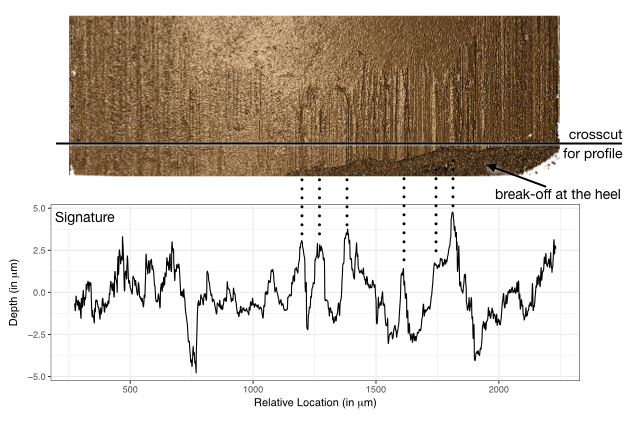
\includegraphics[width=\textwidth]{images/B6-B2-L6-rescaled.png}


\caption{\label{fig:rgl} Image of a bullet land from a confocal light microscope at 20 fold magnification (top) and a chart of the corresponding signature of the same land (bottom). The dotted lines connect some peaks visible in both visualizations.}

\end{figure}

\subsection{Scans for land engraved
areas}\label{scans-for-land-engraved-areas}

Comparisons of striae from bullets are usually based on comparisons of
striae in land engraved areas, which are extracted in form of cross
sections, called \emph{profiles} \citep{aoas,ma2004}. From profiles
bullet \emph{signatures} \citep{chu2013,aoas} are extracted as residuals
of a loess fit or Gaussian filter. Signatures are considered to be noise
free and a good reflection of the key attributes of the raw marking, and
the unique features of a bullet.
\hh{Do you have a reference for the previous sentenced?} A detailed
discussion of the extraction technique for signatures is given in
\citet{aoas}.

\hh{don't split the discussion on the size. between the next paragraph and }
There are two sources of scans for sets from the Hamby study available
to us: scans of Hamby 44 and Hamby 252 are available from the NIST
database \citep{nist}. Hamby 44 has also been made available to us and
has been scanned locally for CSAFE at the Roy J.~Carver High Resolution
Microscopy Facility using a Sensofar confocal light microscope. Scans in
the NIST database are made with a NanoFocus at 20x magnification. The
resolutions of the two instruments are different: the NIST scans are
taken at a resolution of 1.5625 \(\mu m\) per pixel, while the CSAFE
scans are available at a resolution of 0.645 \(\mu m\) per pixel. The
length of an average bullet land from Hamby (9 mm Ruger P85) is about 2
millimeter, resulting in signatures of about 1200 pixels for NIST scans,
and about 3000 pixels for CSAFE scans.

In comparison, scans from the profilometer used by
\citet{chumbley, hadler} were taken at a resolution of about 0.73
\(\mu m\) per pixel. The screw driver toolmarks are about 7 mm in length
\citep{manytoolmarks1}, for a total of over 9000 pixels for the width of
these scans.

This severe limitation in the amount of available data poses the main
challenge in adapting the Chumbley score to matching bullet lands,
because of the resulting loss in power.

\subsection{Potential Challenges in Chumbley Score
Adaptation}\label{potential-challenges-in-chumbley-score-adaptation}

\hh{The Chumbley score allows a separation of a toolmark into raw and normalized digitized versions. Originally, this mechanism is intended to separate between class characteristics and individual markings, however, in the setting of matching bullet striae, we could also use it to separate bullet curvature in profiles from signatures before matching signatures. }

\subsection{The Chumbley Score Test}\label{the-chumbley-score-test}

The Chumbley score algorithm takes input in form of two digitized
toolmarks. The toolmark is in form of \(z(t)\) which is a spatial
process for location indexed by \(t\). \(t\) here denotes equally spaced
pixel locations for the striation marks under consideration,
\(t = 1, ..., T\). Let further \(z(s,t)\) denote the vector of markings
between locations \(s\) and \(t\).

Let \(x(t_1)\), \(t_1 = 1,2,...T_1\) and \(y(t_2)\), \(t_2 = 1,2...T_2\)
be two digitized toolmarks (where \(T_1\) and \(T_2\) are not
necessarily equal). The toolmarks under consideration are potentially
from two different sources or the same source. \(T_1\) and \(T_2\), as
represented above, are the final pixel indexes of each marking and
therefore give the respective lengths of the markings.

In a pre-processing step the two markings are smoothed using a lowess
\citep{lowess} with coarseness parameter \(c\). The purpose of this
smoothing is to remove drift and (sub)class characteristics.

The Chumbley scores is calculated in two phases, namely, an optimization
step and a validation step. In the optimization step, the two markings
are aligned horizontally such that within a pre-defined window of length
\(w_o\) the correlation between \(x(t_1)\) and \(y(t_2)\) is maximized:
\[
\left(t_1^o, t_2^o\right) = \mathop{\arg \max}\limits_{1 \le t_1 \le T_1, 1 \le t_2 \le T_2} \text{cor} \left(x (t_1, t_1 + w_o), y(t_2, t_2 + w_o) \right)
\] This results in an optimal vertical (in-phase) shift of
\(t_1^o - t_2^o\) for aligning the two markings.

In the validation step, two sets of windows of size \(w_v\) are chosen
from both markings (see Figure \ref{fig:win-comparison}). In the first
set, pairs of windows are extracted from the two markings using the
optimal vertical shift as determined in the first step, whereas for the
second set the windows are extracted using a different (out-of-phase)
shift.

\begin{figure}

{\centering 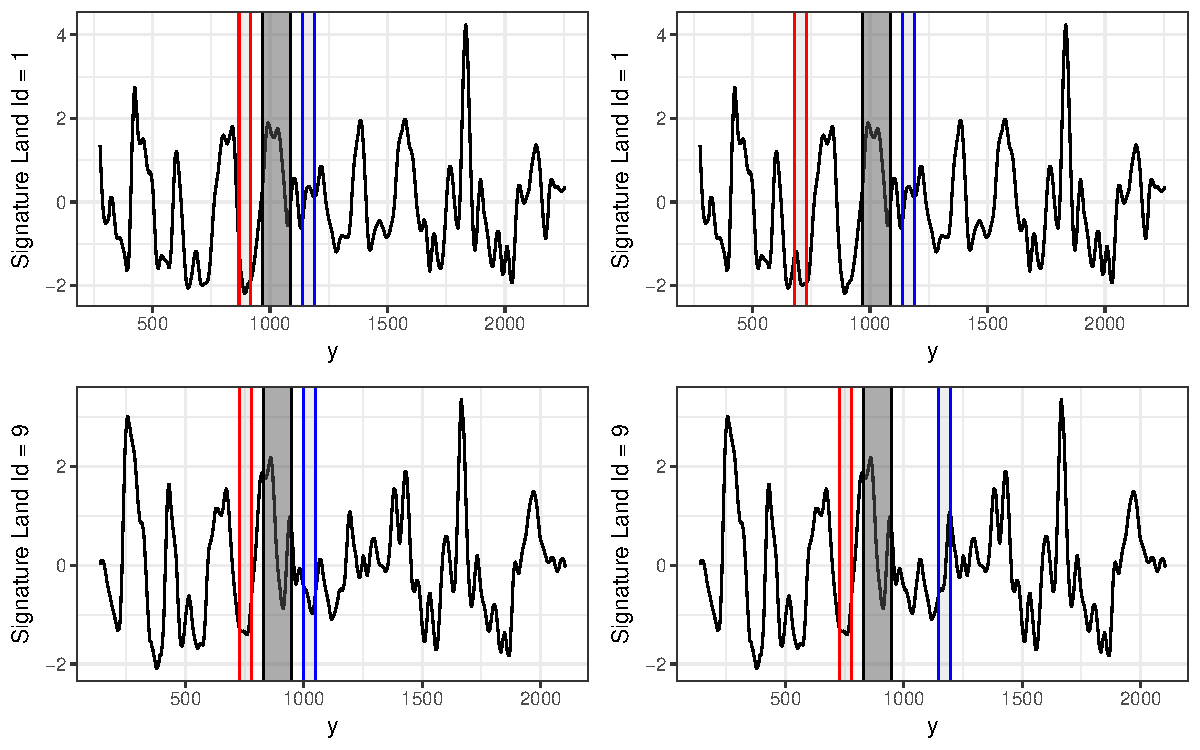
\includegraphics[width=\textwidth]{figures/win-comparison-1} 

}

\caption{Two markings made by the same source. For convenience, the markings are moved into phase on the left and out-of phase on the right. In-phase (left) and out-of-phase (right) samples are shown by the light grey background. The Chumbley-score is based on a Mann-Whitney U test of the correlations derived from these two sets of samples.}\label{fig:win-comparison}
\end{figure}

For both samples the correlations between the pairs of markings is then
calculated. The intuition here is that for two markings from the same
source the correlation for the in-phase sample should be high, while the
correlations of the out-of-phase sample provide a measure for the
base-level correlation for non-matching marks of a given length \(w_v\).
The Chumbley score is then computed as a Mann Whitney U statistic to
compare between in-phase sample and out-of-phase sample. In the original
method proposed in \citet{chumbley} both in-phase and out-of-phase
sample are extracted randomly, whereas \citet{hadler} proposed
deterministic rules for both samples to make the resulting score
deterministic while simultaneously avoiding overlaps within selected
marks to ensure independence.

\section{Testing setup}\label{testing-setup}

\subsection{The Data}\label{the-data}

\hh{Introduce profiles and signatures, as shown in figure \ref{fig:sigs-profiles}.}

\begin{figure}

{\centering 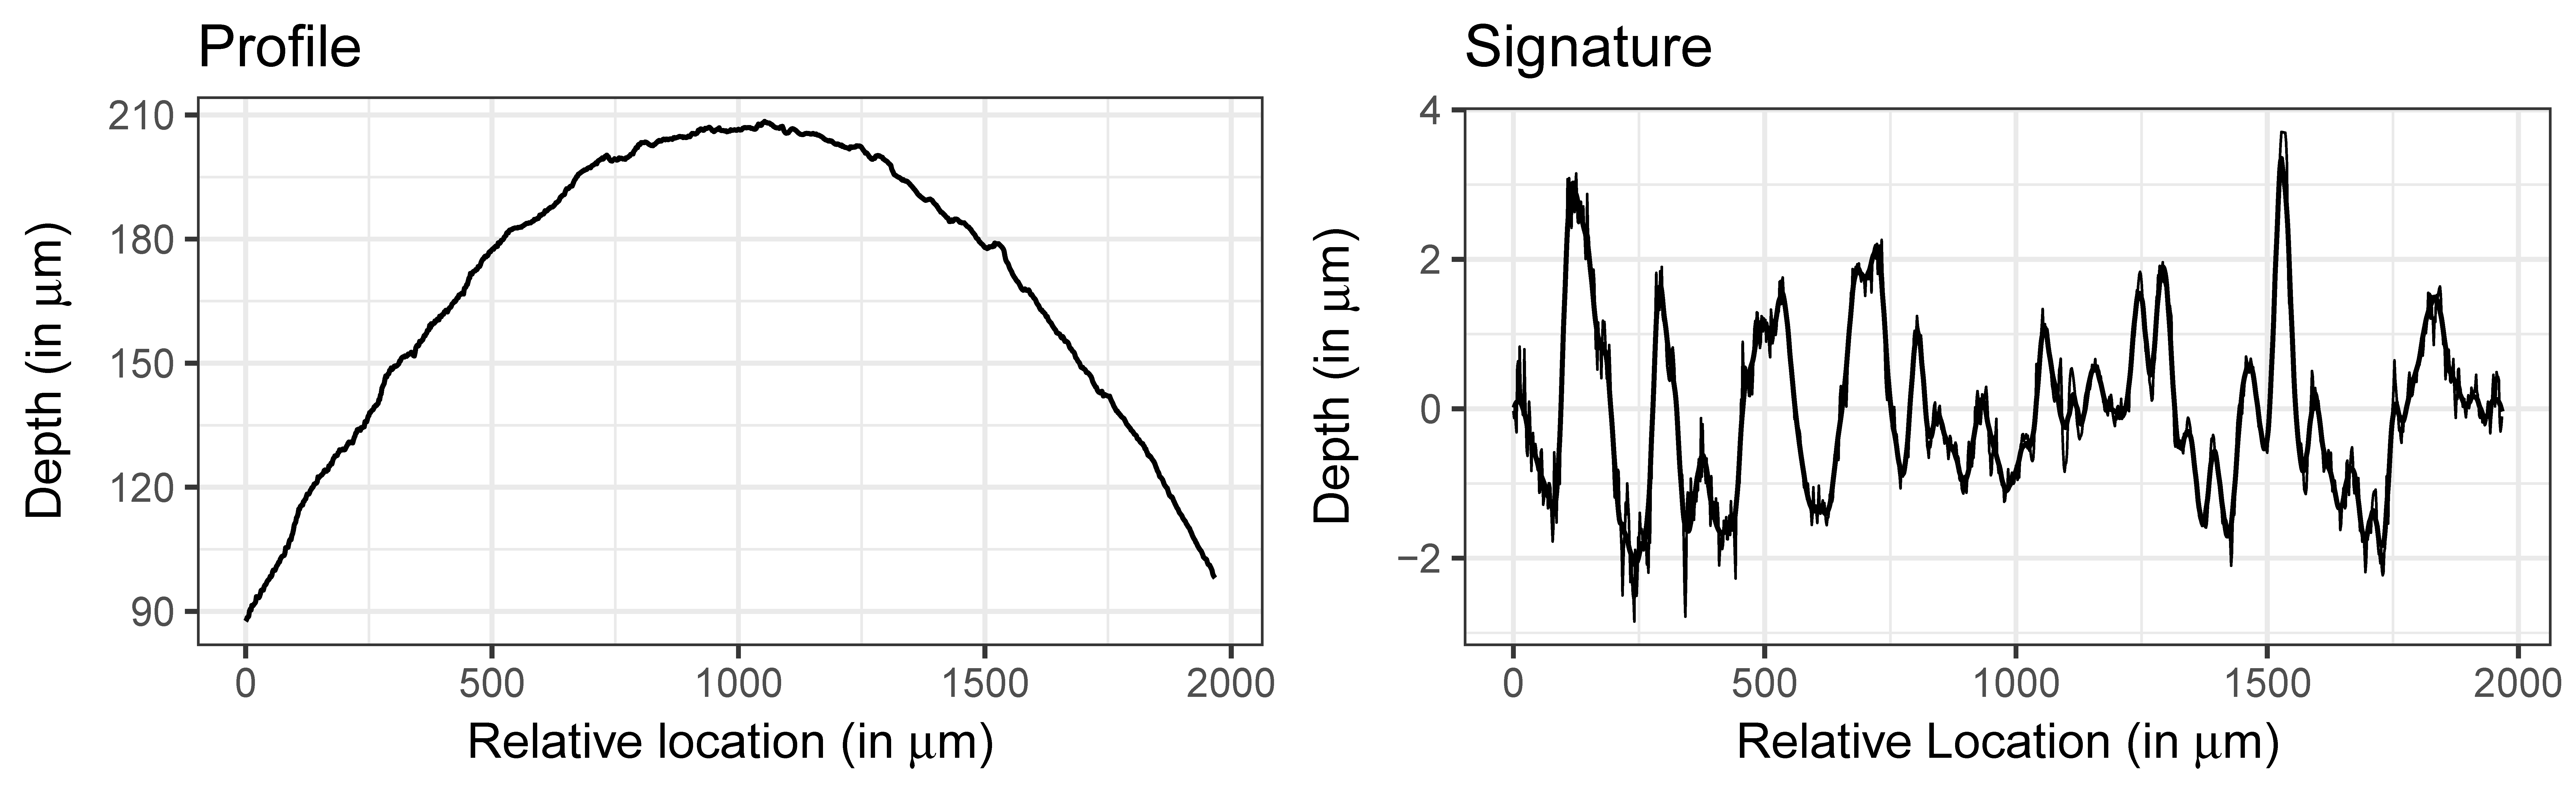
\includegraphics[width=\textwidth]{figures/sigs-profiles-1} 

}

\caption{Bullet land profile (left) and the corresponding signature (right) for one of the lands of Hamby-44.}\label{fig:sigs-profiles}
\end{figure}

Lands for all Hamby-44 and Hamby-252 scans are made available through
the NIST ballistics database \citep{nist} and are considered, here. Both
of these sets of scans are part of the larger Hamby study \citep{hamby}.
Each set consists of twenty known bullets (two each from ten
consecutively rifled Ruger P85 barrels) and fifteen questioned bullets
(each matching one of the ten barrels). Ground truth for both of these
Hamby sets is known and was used to assess correctness of the tests
results.

\hh{Discuss CSAFE scans}

Profiles and signatures were extracted from all scans as described in
\citet{aoas}.

\subsection{Setup}\label{setup}

\hh{using (a) signatures and (b) profiles, run chumbley score across scans from NIST and CSAFE for various settings of $w_o$ and $w_v$ (and coarseness $c$ for profiles).}

We used the adjusted Chumbley method as proposed in \citet{hadler} and
implemented in the R package \texttt{toolmaRk} \citep{toolmark} on all
pairwise land-to-land comparisons of the Hamby scans provided by NIST (a
total of 85,491 comparisons). The settings for optimizing and validating
window sizes, \(w_o\) and \(w_v\), ranged from \(w_o \in [50, 280]\) and
\(w_v \in \{30, 50\}\), see also figure \ref{fig:type2}.

\subsection{Results}\label{results}

\hh{For signatures from NIST scans we see three problems: 
\begin{enumerate}
\item type-2 error rate is at best 30\% for a type-1 error rate of 5\%, which is well above the error rates we see for tool marks from screw drivers, see figure \ref{fig:type2};
\item the observed type-1 error, which generally close to the nominal type-1 error rate, depends on the size of the optimization window: as the window size increases, the observed type-1 error decreases, see figure \ref{fig:type1};
\item the Chumbley-score fails to provide a result for up to 3\% of the cases. The number of failed tests increases linearly in the size used for the window in the optimization step. The rate of failed tests is considerably higher when the two lands are from same source than when the lands are from different sources, see figure \ref{fig:missings}. 
\end{enumerate}
}

Figure \ref{fig:missings} gives an overview of the number of failed
tests, i.e.~tests in which a particular parameter setting did not return
a valid result. This happens e.g.~when the shift to align two markings
is so large, that the remaining overlap is too small to accommodate
windows for validation. The problem is therefore exacerbated by a larger
validation window. Figure \ref{fig:missings}(left) also shows that the
number of failed tests is approximately linear in the size of the
optimization window. Tests also fail at a higher rate than expected when
the markings are from the same source (right). This difference is the
least pronounced around an optimized window size \(w_o\) of around 120.
However, even in this scenario, the number of failed tests for markings
from the same source is about twice as high as expected given the number
of same source and different source pairings in the data set.

\begin{figure}

{\centering 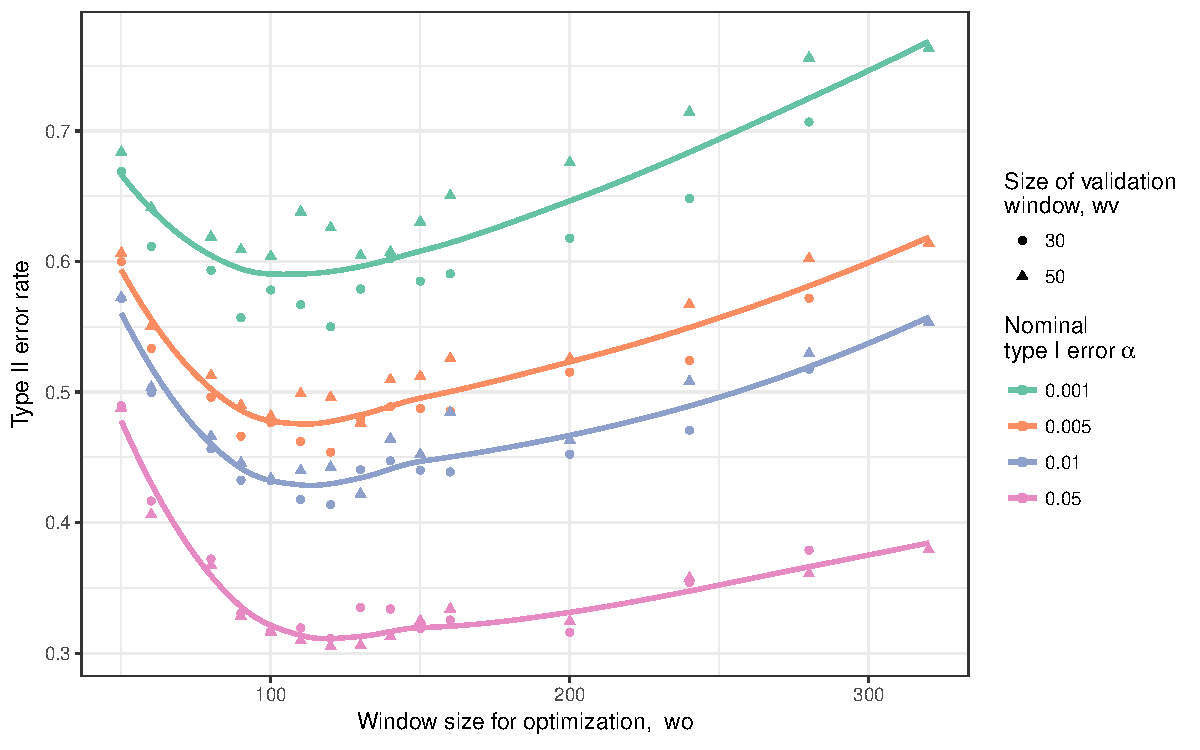
\includegraphics[width=.8\textwidth]{figures/type2-1} 

}

\caption{Type II error rates observed across a range of window sizes for optimization $w_o$. For a window size of $w_o = 120$ we see a drop in type II error rate across all type I rates considered. Smaller validation sizes $w_v$ are typically associated with a smaller type II error.}\label{fig:type2}
\end{figure}

\begin{figure}

{\centering \includegraphics[width=\textwidth]{figures/type1-1} 

}

\caption{Comparison of observed and nominal type I error rates  across a range of window sizes for optimization $wo$. The horizontal line in each facet indicates the nominal type I error rate.}\label{fig:type1}
\end{figure}

\begin{figure}

{\centering 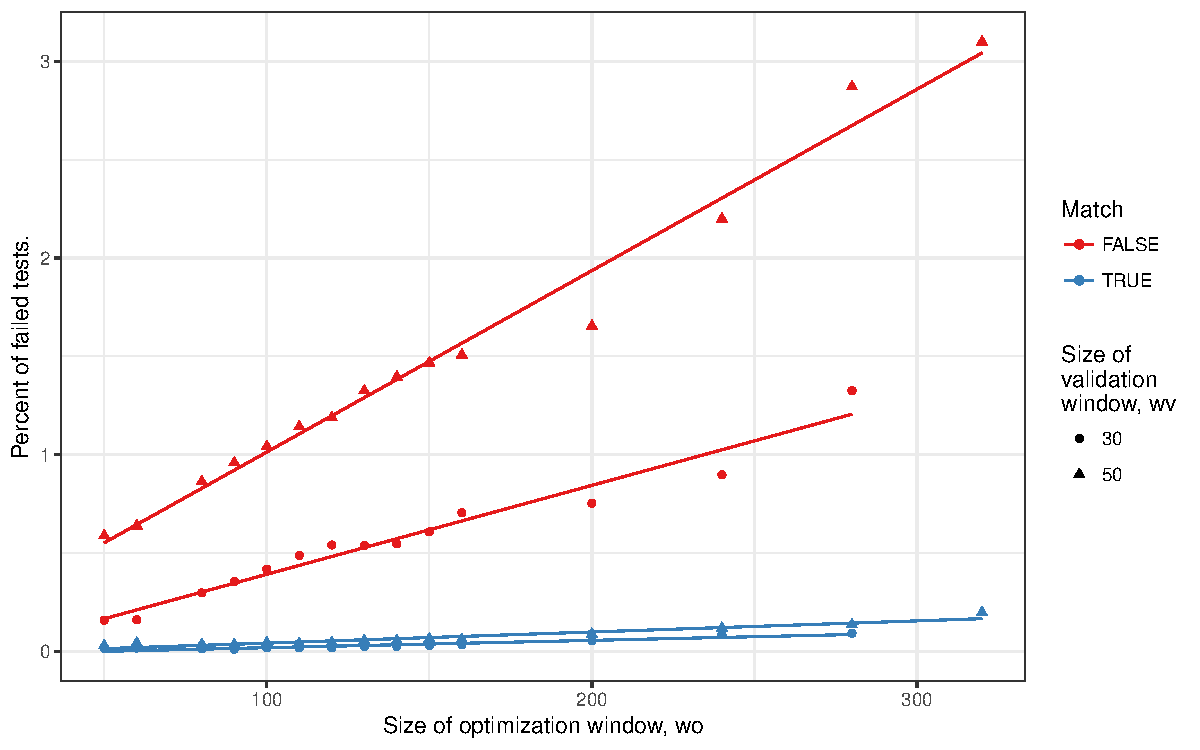
\includegraphics[width=\textwidth]{figures/missings-1} 

}

\caption{The number of failed tests increases with an increase in the size of the optimization window (left). Unfortunately there is also a dependency between failed tests and ground truth. The plot on the right shows the ratio of the number of land pairs from same sources and different sources for failed tests. For small optimization windows and large windows the number of failed tests for same-source land-to-land comparisons is increasing. Even in the minimum, same-source land-to-land comparisons fail at twice the rate that they are expected to based on the ratio of the number of known matches and known non-matches (horizontal line).}\label{fig:missings}
\end{figure}

\section{Results}\label{results-1}

\subsection{Profiles}\label{profiles}

\hh{When dealing with profiles, coarseness is an additional parameter that has to be considered in the matching.}

\hh{XXX We have been operating under a false assumption: smoothing the signature at f=1 DOES change it - see figure \ref{fig:profile-sketch}. We need to re-run some of the results to compare the results against a }

\begin{figure}

{\centering 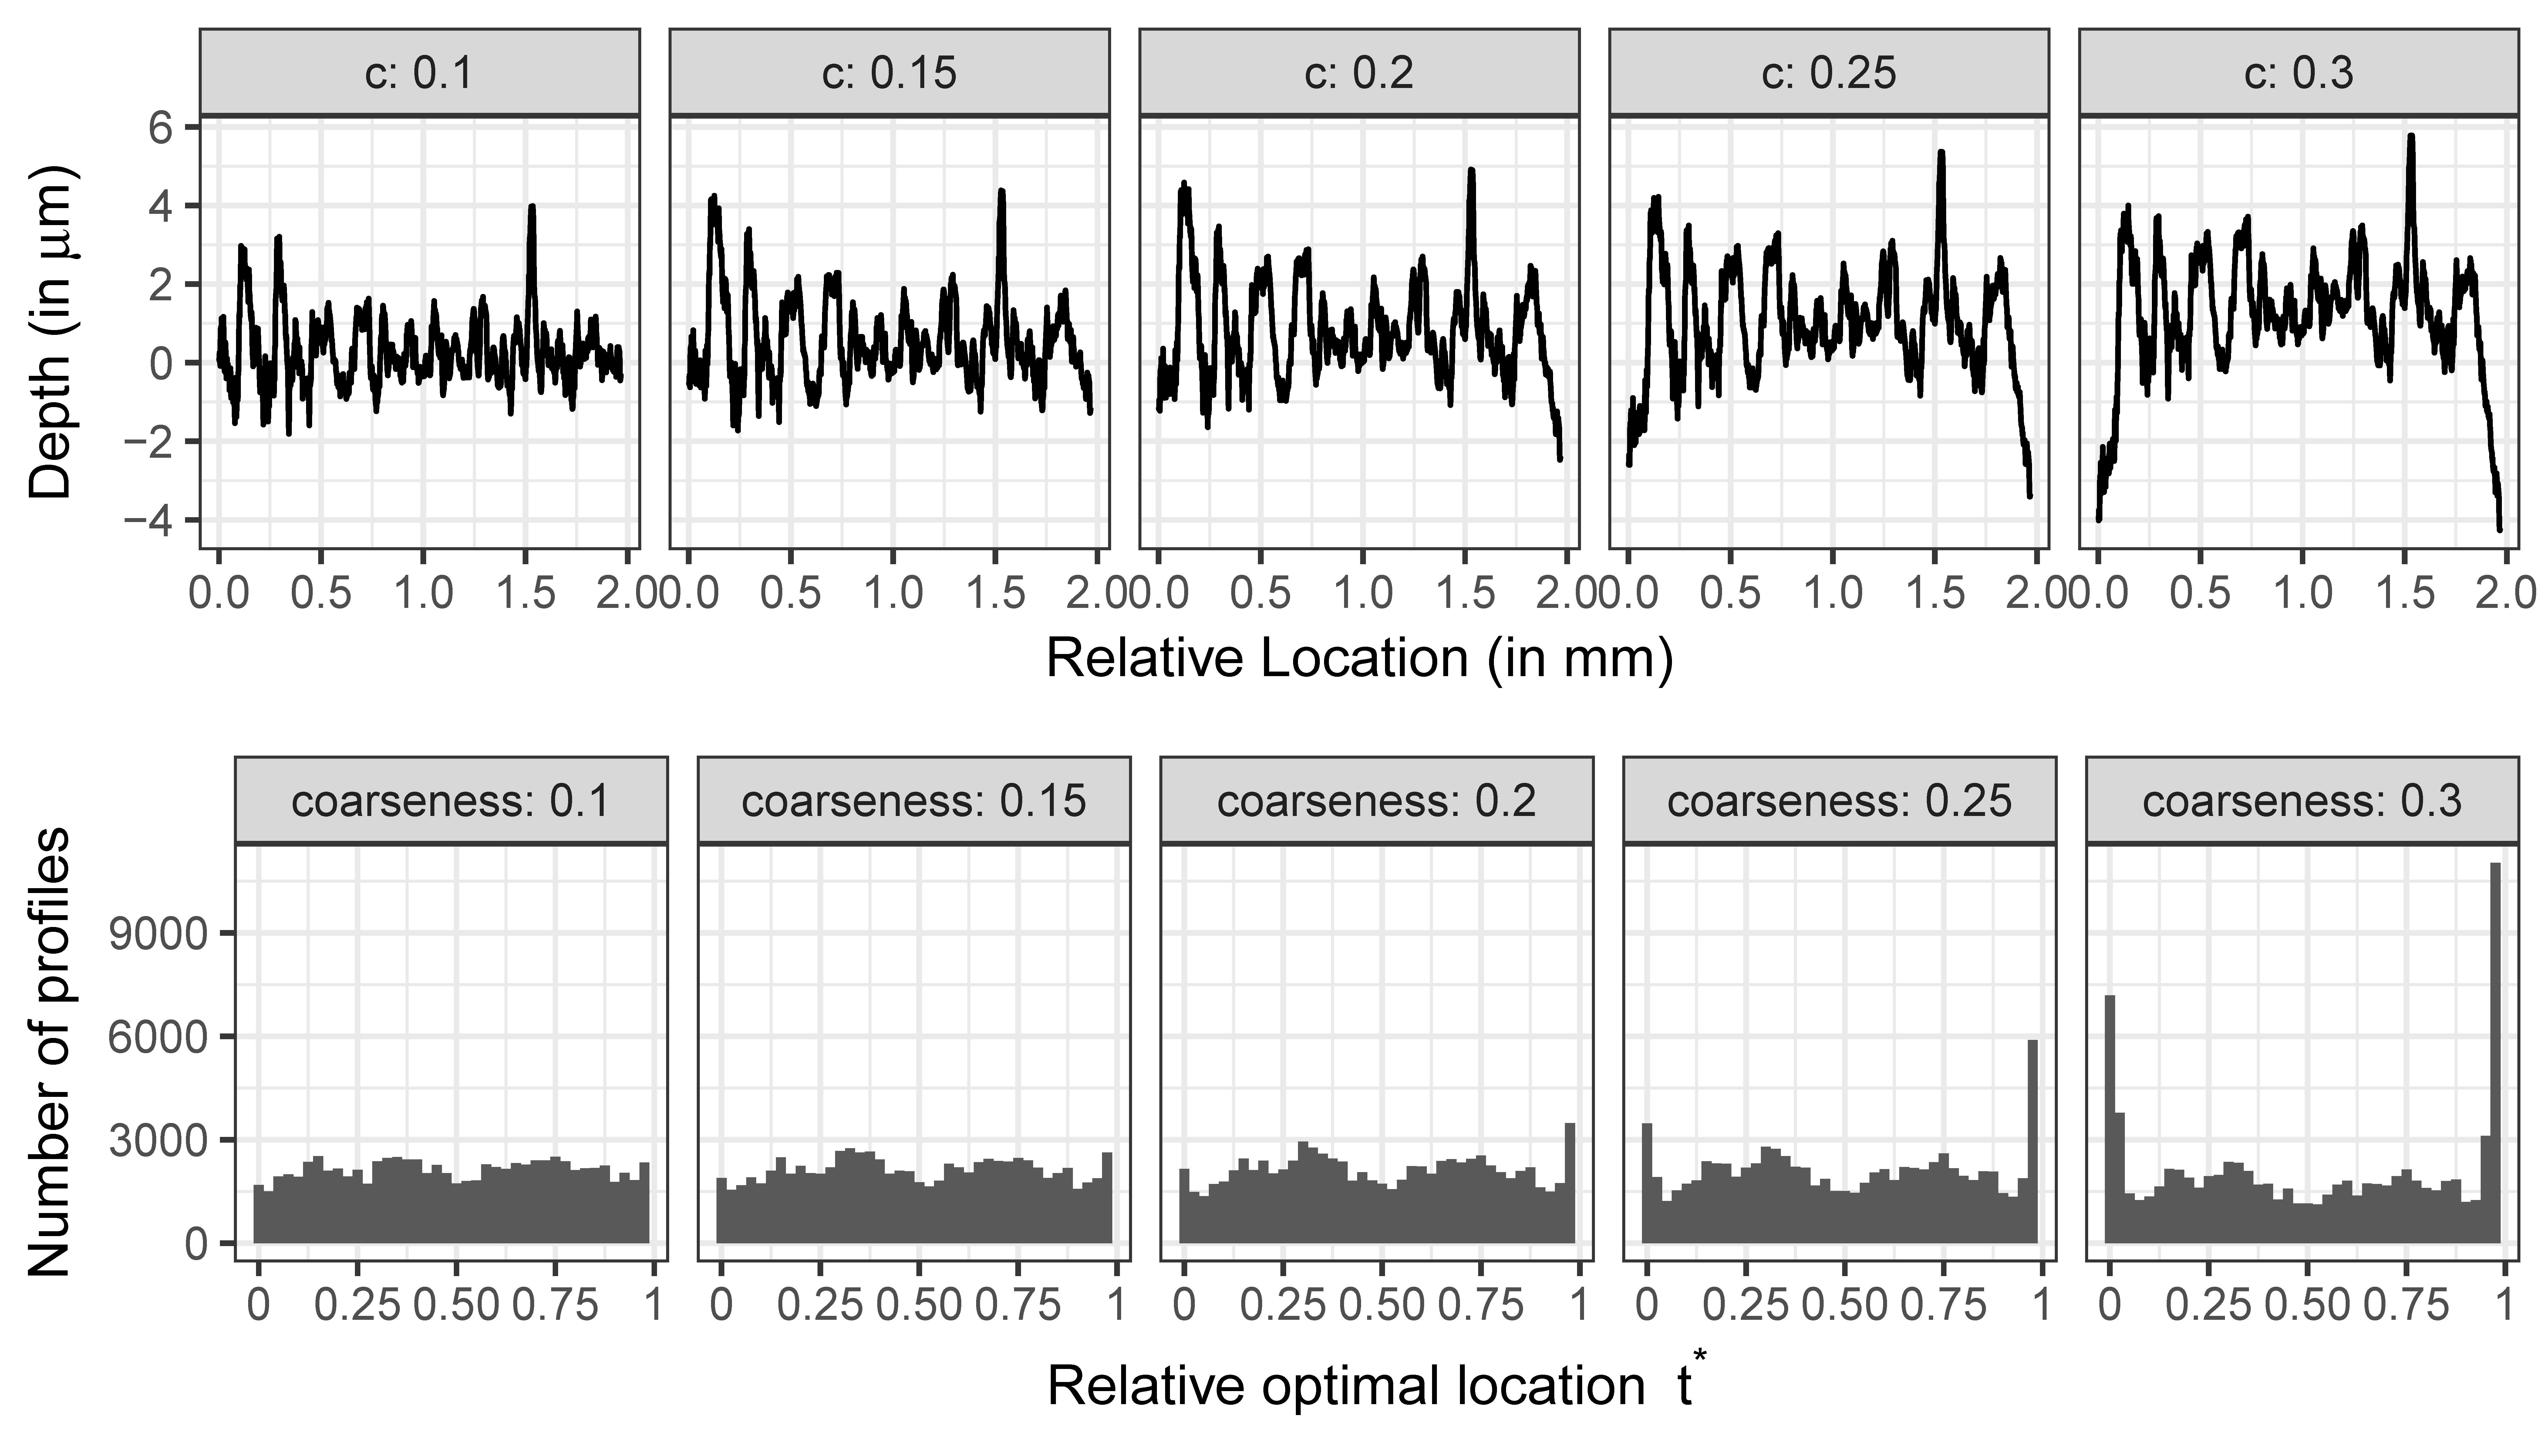
\includegraphics[width=\textwidth]{figures/profile-sketch-1} 

}

\caption{Overview of the effect of different coarseness parameters $c$ on the profile shown in Figure \ref{fig:sigs-profiles}. }\label{fig:profile-sketch}
\end{figure}

\hh{Figure \ref{fig:coarse} shows the type II error rates for profiles using an optimization window $w_o= 120$ and a validation window $w_v = 30$ for varying level of coarseness. The type II error for all nominal levels of  $\alpha$ are the lowest for a coarseness range of 0.20 to 0.35. For the remainder of the analysis we use a fixed value of coarseness of 0.25. }

\begin{figure}

{\centering \includegraphics[width=.6\textwidth]{figures/coarse-1} 

}

\caption{Type II error with respect to coarseness parameter over profiles, $w_o = 120$, $w_v = 30$. Optimal values for coarseness are around $c \approx 0.30$}\label{fig:coarse}
\end{figure}

\begin{table}[ht]
\caption{\label{tab:type2} Type II error rates for profiles and signatures of bullet lands. For profiles, a coarseness value of $c = 0.25$ is used to remove bullet curvature.}
\centering
\begin{tabular}{rlrrrr}
  \hline
optimization && \multicolumn{4}{l}{Nominal type I error rate $\alpha$}\\  
window $w_o$ & source & 0.001 & 0.005 & 0.01 & 0.05 \\ 
  \hline
 30 & profiles & 54.40 & 43.80 & 39.70 & 30.00 \\ 
   30 & signatures & 55.00 & 45.40 & 41.40 & 31.10 \\ \hline
   50 & profiles & 58.50 & 44.40 & 40.70 & 28.70 \\ 
   50 & signatures & 62.60 & 49.60 & 44.20 & 30.50 \\ 
   \hline
\end{tabular}
\end{table}

\section{Conclusion}\label{conclusion}

The results suggest that the Nominal type I error \(\alpha\) value shows
dependence on the size of the window of optimization. For a given window
of optimization the actual Type I error is comparable to the nominal
level for only a select few validation window sizes and for comparable
validation window sizes of 30 and 50 as done here, the actual type I
error does not seem to vary as much as it varies with the optimization
window sizes . A Test Fail, i.e.~tests in which a particular parameter
setting did not return a valid result, happens, when the shift to align
two signatures is so large, that the remaining overlap is too small to
accommodate windows for validation, depends on whether known-match or
known non-matches has predictive value, with test results from different
sources having a much higher chance to fail. On conducting an analysis
of all known bullet lands using the adjusted chumbley algorithm, Type II
error was identified to be least bad for window of validation 30 and
window of optimization 120. In case of unsmoothed raw marks (profiles),
Type II error increases with the amount of smoothing and least for
LOWESS smoothing coarseness value about 0.25 or 0.3. In an effort to
identify the level of adaptiveness of the algorithm, comparisons were
made between signatures and profiles. Their comparison with respect to
validation window size for a fixed optimization window size suggested
that, profiles have a total error (i.e all incorrect classification of
known-matches and known non-matches) greater than or equal to the total
error of signatures for all sizes of validation window. Profiles also
fail more number of times than signatures in a test fail (for different
coarseness keeping windows fixed and also for different validation
windows keeping coarseness fixed) which lets us conclude that the
behaviour of the algorithm for the profiles instead of pre-processed
signatures is not better. Finally it should be noted that the current
version of the adjusted chumbley algorithm seems to fall short when
compared to other machine-learning based methods \citet{aoas}, and some
level of modification to the deterministic algorithm needs to be
identified and tested that would reduce the number of incorrect
classifications.

\section{Appendix}\label{appendix}

\begin{appendix}

On the other hand Figure \ref{fig:prof_missings} (b) shows if the coarseness level set in the chumbley agorithm has any effect on the signatures, which are pre-processed and already smoothed to a certain extent. From Figure \ref{fig:prof_missings} (b) we can notice that for different nominal $\alpha$ levels, the type II error fluctuates slightly but does not change much, thereby helping us conclude that the coarseness levels set in the LOWESS smoothing in the chumbley alggorithm does effect the type II error much for signatures.

\subsection{Comparison of profiles and signatures}

Another reason for failed tests can be incorrect identification of maximum correlation windows in the optimization step as seen in figure \ref{fig:prof_missings}(d) because of the level of smoothing, as too much smoothing would subdue intricate features that might otherwise help in the correlation calculations and correct identification of maximum correlation windows irrespective of the size. This would again cause a simiar effect as explained for figure \ref{fig:missings} with validation windows, irrespective of size, during the shifts end up at the ends of the markings resulting in an invalid calculation and failed comparison attempt. 

In figure \ref{fig:prof_missings}(d) and (f), we compare profiles and signatures on the basis of number of failed tests. The profiles chosen for figure \ref{fig:prof_missings}(f) have a constant coarseness of 0.25 and window of optimization as 120. The signatures in this case are not smoothed using the chumbley algorithm step of LOWESS smoothing. Instead signatures are used as calculated by \citet{aoas}. The smoothing in these signatures were determined and fixed on the basis of their performance in the random forest based algorithm proposed by \citet{aoas}. The comparison of profiles and signatures with variation of validation window size therefore is made on even footing. The trends are similar to figure \ref{fig:missings} in the sense that for known non-matches the number of failed tests are more for both signatures and profiles and increasing linearly with the validation window size. The problem is however, worse for profiles which has higher number of failed tests than signatures for all validation windows.

The total error for different validation window sizes for signatures and profiles can be seen in figure \ref{fig:prof_missings} (e).The optimization window size is 120 and profiles are calculated at a default 0.25 coarseness level while signatures as before are not smoothed again in the modified chumbley algorithm. We can see that the total error is always higher for profiles as compared to signatures for all sizes of validation window. 







\begin{figure}

{\centering \includegraphics[width=\textwidth]{figures/prof_missings-1} 

}

\caption{Row 3:  Total error and Number of failed tests by the window validation size, wv, and ground truth, Row 2: Total error and Number of failed tests with Coarseness for both profiles and signatures, Row 1: Type II error for different coarseness levels as used in the modified chumbley algorithm for profiles and signatures}\label{fig:prof_missings}
\end{figure}
\end{appendix}

\bibliographystyle{agsm}
\bibliography{bibliography}

\end{document}
